\chapter{Diseño e Implementación}
\title{Diseño e Implementación}
\label{cap:DisenoEImplementacion}
Este proyecto se realiza atendiendo a dos partes, ambas muy importantes y claramente diferenciadas. Por una parte, se ha creado el diseño del prototipo de cliente y por otra parte se ha elaborado el boceto de la interfaz con su posterior diseño de interfaz de usuario.

\section{Diagrama del Modelo Conceptual}
El diagrama del modelo conceptual nos ofrece una idea de cómo se encuentra interrelacionadas las diferentes entidades del sistema.
\begin{figure}[htb]
\centering
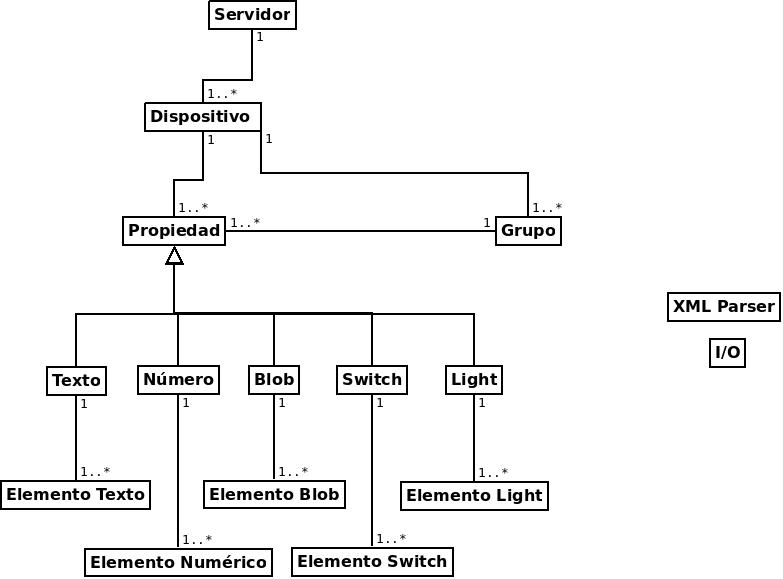
\includegraphics[width=0.8\textwidth]{./imagenes/diagramaConceptual}
\caption{Modelo Conceptual} \label{fig:diagramaConceptual}
\end{figure}

Como se puede observar en el diagrama, en un servidor se pueden encontrar uno o muchos dispositivos conectados en él.
A su vez, un dispositivo puede tener un conjunto de propiedades y un conjunto de grupos. Las propiedades solamente pueden pertenecer a un grupo concreto.\\
Cada propiedad es solamente de un tipo, que puede ser \textit{text}, \textit{number}, \textit{switch}, \textit{blob} y \textit{light}. A su vez, la propiedad puede tener uno o muchos elementos de dicha propiedad.\\

Por último, hay que destacar que se han creado las entidades \textit{XML Parser} y \textit{I/O}, para el parseo de los mensajes enviados por el servidor en \textit{XML} y para la entrada y salida, respectivamente.


\section{Diseño del Prototipo del Cliente}
El diseño del prototipo del cliente es la pieza fundamental del proyecto ya que sobre dicho prototipo giran todas las cosas.\\

La función principal del prototipo es permitir conectarnos con cualquier servidor INDI y una vez que establecemos la conexión, mediante el WebSocket, es fundamental que la comunicación se establezca de forma continua con el fin de recibir los diferentes dispositivos que se encuentran conectados con el servidor en concreto y así poder intercambiar mensajes con los parámetros que se van modificando en ambas partes.

\subsection{Métodos en el Fichero \textit{connection.js}}
El cometido de estos métodos es establecer la conexión con el servidor.
También, en ese archivo, se pueden encontrar los métodos para poder realizar el envío de valor de los parámetros modificados, ya sea de tipo \textit{text}, \textit{number}, \textit{switch} o \textit{blob}, al servidor mediante el \textit{WebSocket}, que se crea en el momento de la conexión.

\subsection{Métodos en el Fichero \textit{parserDefVector.js}}
Este fichero se establece en dos grandes bloques. En primer lugar, se encuentran los métodos mediante los cuales se va creando la interfaz con los datos que se reciben del fichero XML, como pueden ser, entre otros, los nombres de los dispositivos, los nombres de las propiedades, los apelativos de los grupos de las propiedades, los valores que tienen dichas propiedades, etc. En segundo lugar, se hallan las funciones auxiliares para crear dicha interfaz y que sirven de apoyo a los métodos de análisis y parseo de las propiedades.\\

Una vez que llegan esos datos se crean las diferentes ventanas que corresponden a cada dispositivo siempre y cuando estos dispositivos no estén ya creados.
Tanto para las propiedades de \textbf{texto} como para las de \textbf{número} se realiza el mismo proceso.\\

A continuación, se pone una bombilla del color correspondiente según el estado que envíe el fichero XML que proviene del servidor, y el nombre de la propiedad. Este conjunto se ha denominado \textit{propertyBox}.
Seguidamente, mediante el parseo del fichero XML, se va recorriendo cada uno de los nodos que lo van formando y para cada uno de ellos se muestra el nombre que viene descrito mediante el campo \textit{label} y su correspondiente valor del nodo. Al conjunto formado por el nombre y el valor se le ha denominado \textit{elementBoxContainer}.\\

Posteriormente, y según el tipo de permiso que tenga esa propiedad, se pone o no el botón de actualizar para que en el futuro se puedan modificar los campos y poder así enviarle el mensaje al servidor.\\

Por último, se añade a las diferentes pestañas la propiedad, según el grupo al que pertenece la propiedad que se está analizando.\\

Para el análisis y posterior parseo de la propiedad \textbf{\textit{switch}} se sigue el mismo itinerario con el que se ha procedido en los \textit{text} y en los \textit{number}, con la diferencia de que en la parte del \textit{elementBoxContainer}, se hacen diferentes tipos de llamadas para cada una de las diferentes reglas  que pueden contener las propiedades \textit{switch}:
\begin{itemize}
  \item \textbf{\textit{One Of Many:}} se crea un desplegable que siempre obliga al usuario a tener una opción seleccionada en ella.
  \item \textbf{\textit{At Most One:}} se crea un desplegable que permite al usuario si así lo desea o le es factible, solo seleccionar una de todas las opciones que se muestran en él.
  \item \textbf{\textit{Any Of Many:}} se crea un conjunto de opciones que le permitirán al usuario seleccionar todas las que se deseen.
\end{itemize}
Según el tipo de permiso que tenga esa propiedad, se dispone o no, el botón de actualizar para que en el futuro se puedan modificar los campos y poder enviarle el mensaje al servidor.\\

Para el análisis y parseo de la propiedad \textbf{\textit{blob}}, se ha seguido también el mismo procedimiento que en las diferentes propiedades pero en este caso, se ha hecho una pequeña variante en la parte del \textit{elementBoxContainer}. Dentro de ella se muestra, igualmente, el nombre y el valor de la propiedad y además, se añaden dos campos nuevos que son el tamaño del \textit{blob} y su correspondiente formato.
De igual forma, en su parte derecha, y siempre dependiendo  del tipo de permiso que corresponda, se añade o no el botón de actualizar para enviar los datos al servidor.\\

En último lugar, hay que decir que en la parte del análisis y su correspondiente parseo sobre la propiedad \textbf{\textit{light}}, se realiza lo mismo que en las diferentes propiedades salvo en el \textit{elementBoxContainer} que se añade el nombre de la propiedad y el color de la bombilla correspondiente al valor que se envía en ese nodo.\\

Hay que destacar que esta propiedad es siempre del tipo solo lectura y por tanto, no se agregará nunca un botón ya que no se pueden cambiar los valores que tiene.\\

Por otra parte, hay que destacar los métodos auxiliares para la creación del interfaz. Estos métodos son de igual o más importancia que los anteriores ya que sin ellos no se podrían crear las ventanas, poner los diferentes tipos de interruptores o incorporar las diferentes pestañas a las ventanas de los dispositivos.\\

\subsection{Métodos en el Fichero \textit{parserSetVector.js}}
Están constituidos por un total de cinco métodos, uno para cada una de las diferentes propiedades que dispone INDI.
La función principal de estos cinco métodos es común a todos y es la de almacenar los diferentes valores que se cambian en el prototipo de cliente para poder enviárselos al servidor.
Actualmente, en el prototipo, la función de envío se está realizando sobre los propios botones, sobre los desplegables o sobre los \textit{checkbox} que se han ido creando dinámicamente en el fichero anterior. En esos botones se realiza la llamada que corresponda al envío según la propiedad y se hace todo el envío desde el fichero connection.js como se ha mencionado anteriormente.

\subsection{Métodos en el Fichero \textit{parser.html}}
Es el punto de partida de todo el proceso. Desde ahí se establece la conexión con el servidor y se crea un bucle mediante el cual se va enviando la información a las diferentes funciones según el tipo de propiedad que se esté recibiendo o enviando.
También dispone de un conjunto de funciones auxiliares que son comunes tanto a \textit{parserDefVector.js} como a \textit{parserSetVector.js}. Estas pueden ser, por ejemplo, el obtener el nombre de las funciones o conseguir lograr el tipo de bombilla a poner, entre otras.

\section{Bocetos de la Interfaz}
La interfaz de usuario es el medio con que el usuario puede comunicarse, en este caso, con la computadora mediante su navegador y comprende todos los puntos de contacto entre el usuario y el equipo. Por regla general, suelen ser fáciles de entender y fáciles de interactuar con ellas, aunque en el ámbito de la informática es preferible referirse a ellas como que suelen ser “amigables e intuitivas” porque es complejo a la vez que  subjetivo, nombrarlas con el adjetivo “fácil” \cite{IU}.\\

A lo largo de cada una de las diferentes iteraciones del proceso se han ido mejorando las interfaces ya que se ha ido incrementando el número de elementos y por tanto, cada vez había que hacer la interfaz con un grado de dificultad añadido.\\

En la primera iteración se elaboró todo el diseño en papel para ir constituyendo un esquema de lo que sería la futura la interfaz de usuario.\\
\begin{figure}[htb]
\centering
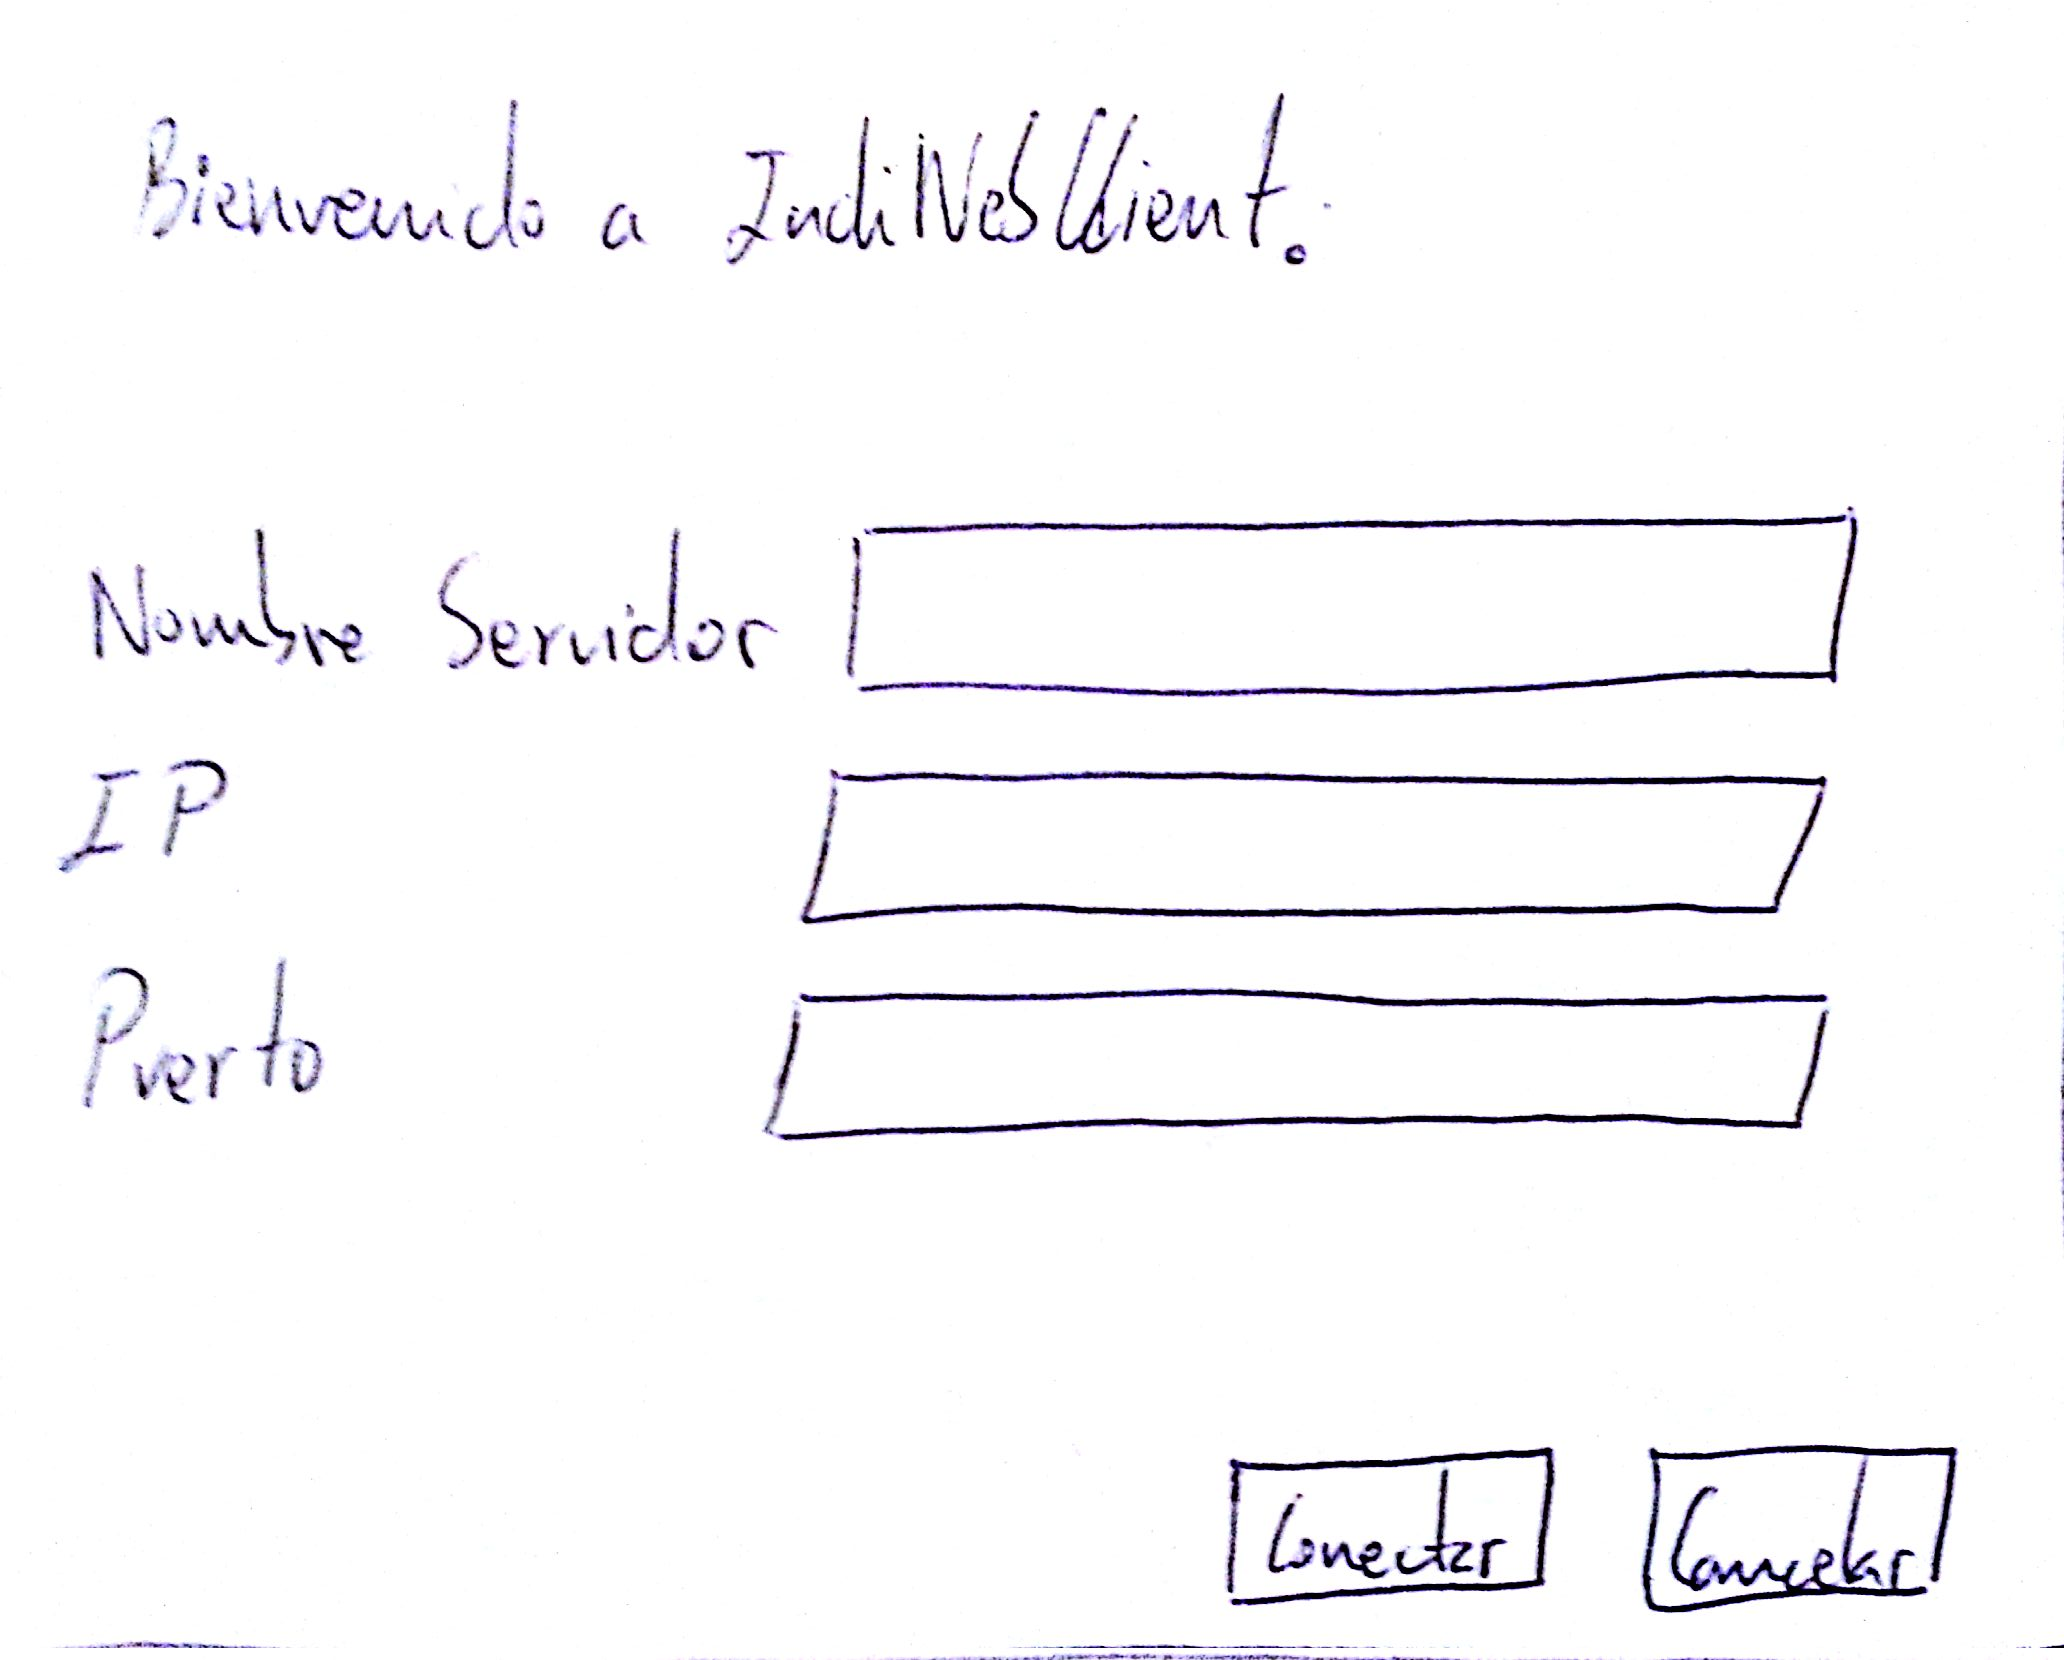
\includegraphics[width=0.7\textwidth]{./imagenes/boceto1}
\caption{Boceto de la Interfaz (I)} \label{fig:boceto1}
\end{figure}

\begin{figure}[htb]
\centering
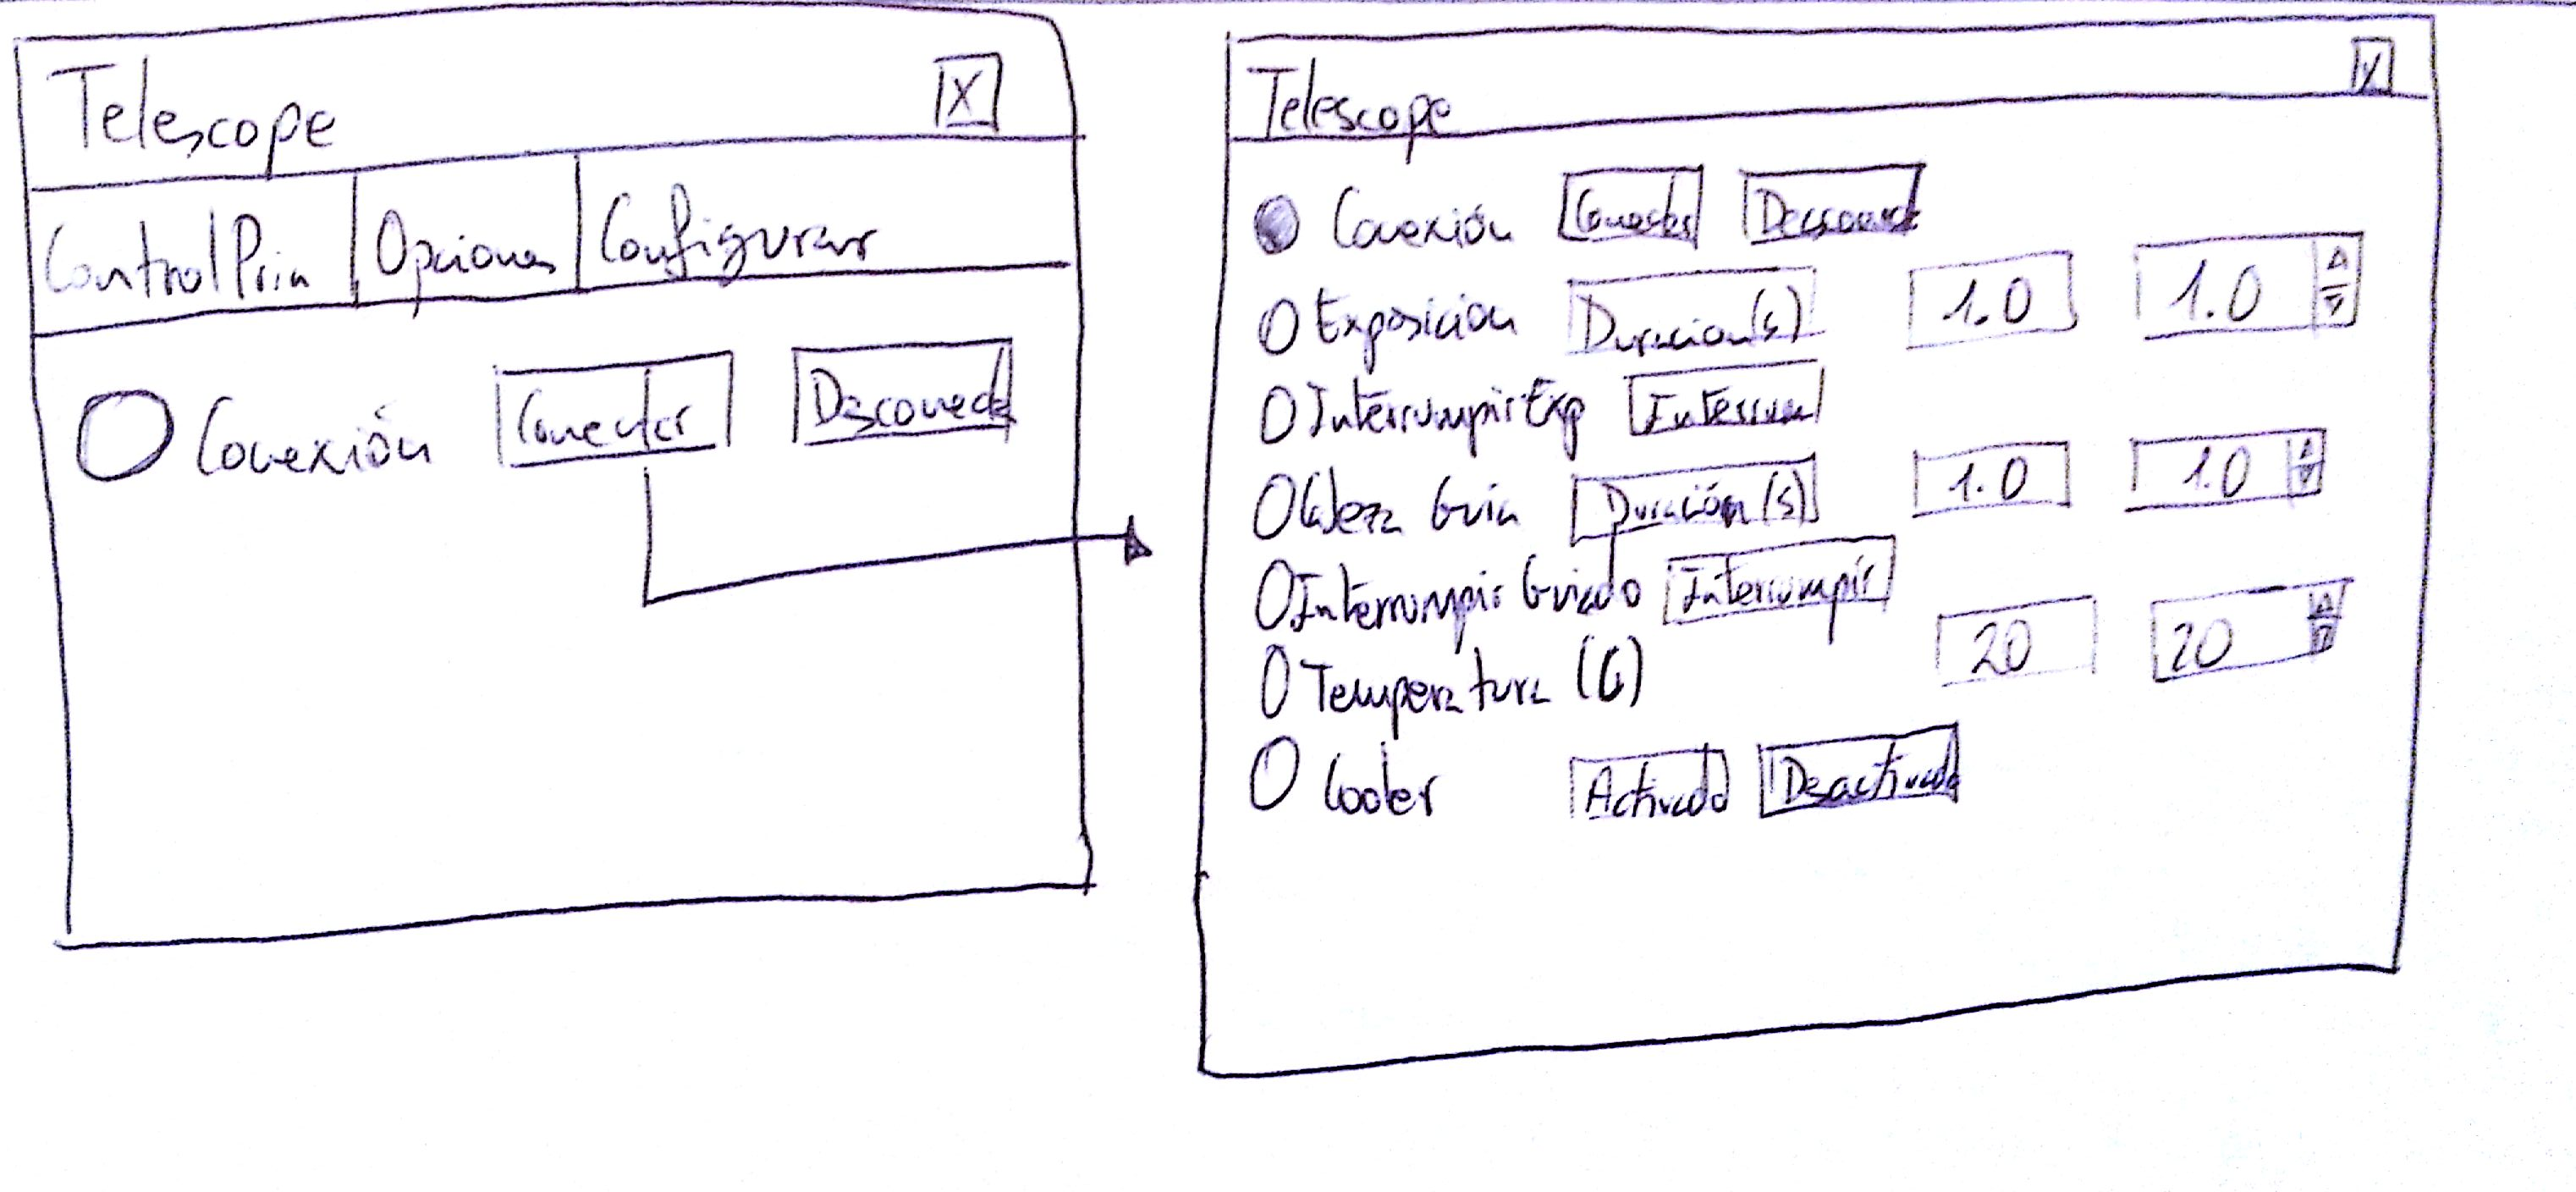
\includegraphics[width=1\textwidth]{./imagenes/boceto2}
\caption{Boceto de la Interfaz (II)} \label{fig:boceto2}
\end{figure}

Seguidamente, y en las iteraciones posteriores, se comenzó a plasmar el trabajo del papel en el navegador comenzando a crear las primeras ventanas para ir proyectando como colocar los diferentes elementos que las iban a integrar.

\begin{figure}[htb]
\centering
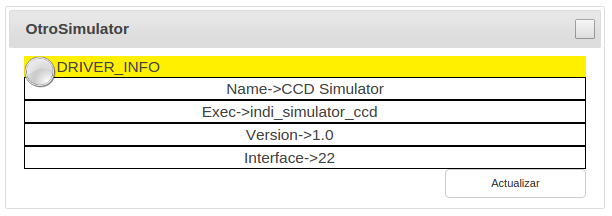
\includegraphics[width=1\textwidth]{./imagenes/primerasVentanas1}
\caption{Primeras Ventanas de la IU (I)} \label{fig:primerasVentanas1}
\end{figure}

\begin{figure}[htb]
\centering
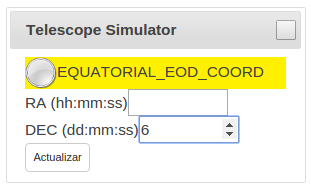
\includegraphics[width=0.7\textwidth]{./imagenes/primerasVentanas2}
\caption{Primeras Ventanas de la IU (II)} \label{fig:primerasVentanas2}
\end{figure}

Posteriormente, se consiguió el diseño final de la interfaz del prototipo del cliente web.\\ \\

\begin{figure}[htb]
\centering
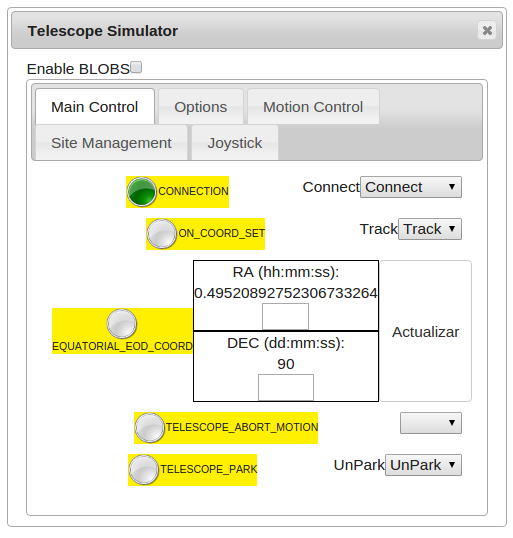
\includegraphics[width=0.8\textwidth]{./imagenes/interfazActual}
\caption{Interfaz de Usuario Actual de Dispositivo} \label{fig:interfazActual}
\end{figure}

\section{Diseño de la Interfaz}
Para obtener unos mejores resultados, se han ido desarrollando las interfaces por separado:
\begin{itemize}
  \item Interfaz de conexión.
  \item Interfaz de propiedad.
  \item Interfaz de grupo de elementos.
  \item Interfaz de dispositivo.
\end{itemize}

\subsection{Interfaz de Conexión}
Se define como la pantalla principal del prototipo de cliente. En ella se muestran dos cuadros de texto para introducir la IP y el puerto del servidor con el que se desea conectar.

\subsection{Interfaz de Propiedad}
Es una interfaz que tendrá, aproximadamente para cada propiedad, la misma estructura.
En la parte izquierda se observa como aparece la bombilla del estado de la propiedad y seguidamente su nombre. A continuación, se encuentra el nombre y el valor de la propiedad o nombres y valores, dependiendo de si tiene más de uno. Por último se encuentra el botón de actualizar, para el caso de que su permiso lo permita.\\

Para los \textit{switch} en la parte central, seguido de la bombilla y el nombre, se encontrará el desplegable con las diferentes opciones o casillas para marcar, según el caso de  su regla de \textit{switch}, ya  sea una u otra.\\

Para los \textit{blob}, su parte central, estará formada por el nombre y el valor, y además existirán dos campos extra que serán el tamaño y el formato del propio \textit{blob}.\\

Para los \textit{light}, en su parte central, se encontrará una o más bombillas con su correspondiente nombre cada una.

\subsection{Interfaz de Grupos de Propiedades}
La interfaz del grupo de propiedades comprende las diferentes pestañas según se agrupan las propiedades. Cuando llega un mensaje en \textit{XML} del servidor se analiza y se comprueba si para el dispositivo que ha enviado el mensaje hay ya creada una ventana, que en caso de no existir, se crea y a continuación el grupo se almacena como una pestaña en la cual irán todas las propiedades de ese grupo.
Se comprueba si la pestaña correspondiente a ese grupo existe y en caso de existir, se muestra la propiedad en esa pestaña. En caso contrario, si se da la circunstancia de que no existiera se crea una nueva pestaña y se muestra en ella la propiedad que envía en ese momento el servidor.\\

\subsection{Interfaz de Dispositivo}
Se entiende por interfaz de dispositivo la ventana encargada de mostrar toda la información del dispositivo conjuntamente con las diferentes interfaces precedentes descritas. En ella se pueden encontrar las diferentes propiedades de un dispositivo en cada una de las pestañas según correspondan a un grupo o a otro. Esta interfaz es la que se muestra cuando se realiza la conexión con el servidor INDI para cada uno de los dispositivos conectados. Es la interfaz que tiene mayor importancia puesto que en ella se muestra toda la información correspondiente al dispositivo.


\section{Implementación}
\subsection{Licencia}
Una de las principales características de este proyecto es que, desde un primer momento, se pensó en la elección de \textit{Software Libre} como herramienta y soporte para su desarrollo y posterior utilización. Se ha elegido  la licencia \textbf{GPL v3} por los siguientes motivos:

\begin{itemize}
  \item Es \textit{Software Libre}.
  \item Obliga a redistribuir con la misma licencia.
  \item Está aprobada por \textit{Open Source Initiative}.
  \item Se compromete y obliga a poder disponer del material de forma ilimitada y gratuita para toda aquella persona que lo solicite.
\end{itemize}

\subsection{Desarrollo de Código}
Para todo el desarrollo del código se ha utilizado el editor de textos y código Sublime Text\cite{Sublime}.
Las razones que hemos tenido para hacer esta elección han sido las siguientes: el tener un tamaño muy reducido, poseer un arranque casi inmediato y poder ampliar su funcionalidad a través de \textit{plugins}.

Este editor de textos y código no es gratuito. Eso es cierto, sin embargo, para el desarrollo de este proyecto que se presenta, he utilizado una versión de prueba que es de tiempo ilimitado \cite{BeneficiosSublime}.\\

Por otra parte, y para tener un control de versiones se ha utilizado \textit{Git}, así como para guardar los datos se ha recurrido al servicio \textit{GitHub}\cite{GitHub}.

Todo el código fuente se puede encontrar en el \href{https://github.com/PabloTorrecillas/IndiWebClient}{repositorio del proyecto} (https://github.com/PabloTorrecillas/IndiWebClient/).
